\documentclass{beamer}
\usepackage{movie15}
\usetheme{AnnArbor}
\usecolortheme{dolphin}
\setbeamercolor*{frametitle}{bg=white,fg=structure.fg}
\title{Exploring the parallelisation of the Large Eddy Simulation using MPI and
the Glasgow Model Coupling Framework}
\author{Gordon Reid - 1002536r}
\date{April 22, 2015}
\newif\ifplacelogo
\placelogofalse
\logo{\ifplacelogo
\includegraphics[width=2cm]{images/ARCHIE-WeSt_logo1.jpg}\vspace{180pt}\fi}
\begin{document}
\frame{\titlepage}
\frame{\tableofcontents}
\section{LES}
\subsection{What is the LES?}
\frame{
    \frametitle{What is the LES?}
    \includemovie[poster,repeat,controls,text={Click to play}]
                 {6cm}{4cm}{videos/pressure_at_75_over_t.avi}
    \begin{itemize}
        \item Large Eddy Simulation models turbulent flows in urban environments
        \item Originally in FORTRAN 77, automatically ported to Fortran 95
        \item Single-threaded, candidate for parallelisation
        \item Operates over 3D area, outputs 4D arrays to netCDF files
        \item Video shows evolution of pressure over time for a 2D slice of area
    \end{itemize}
}
\subsection{Parallelisation Techniques}
\frame{
    \frametitle{Parallelisation Techniques}
    \begin{itemize}
        \item Using MPI for shared- and distributed-memory parallelism
        \item Using GMCF for shared-memory parallelism
        \item MPI acts as baseline to compare GMCF with
    \end{itemize}
    \begin{itemize}
        \item LES instances organised into 2D grid, each taking slice of total area
        \item Need communication to distribute and gather whole arrays
        \item At each time step, side flows and halos need to be exchanged
        \item Also global reductions to get the min, max, and sum of scalars
    \end{itemize}
}
\section{GMCF}
\subsection{What is GMCF?}
\frame{
    \frametitle{What is GMCF?}
    \begin{itemize}
        \item New model coupling framework: Glasgow Model Coupling Framework
        \item Model coupling allows to separate applications to interact
        \item LES can be coupled to the Weather Research and Forecasting model
        \item Shown to improve accuracy of results
        \item Existing model coupling frameworks can require a lot of work to use
        \item GMCF aims to automate some of the model coupling work
        \item Existing frameworks not multicore or heterogeneous aware, GMCF is
        \item GMCF uses a load balancing technique to limit node communication
    \end{itemize}
}
\subsection{GMCF Architecture}
\frame{
    \frametitle{GMCF Architecture}
    \includegraphics[width=0.5\textwidth]{images/gmcfArchitecture.png}
    \begin{itemize}
        \item GMCF uses threads, one per model instance
        \item Each instance has its own GMCF Tile that holds all data for it
        \item GMCF has a concept of packets, instances communicate via packets
        \item Packets for requesting data, sending pointers to data, and more
        \item Received packets are demultiplexed into per type per sender FIFOs
    \end{itemize}
}
\placelogotrue
\section{Evaluation}
\frame{
    \frametitle{Evaluation}
    \begin{itemize}
        \item MPI and GMCF for shared-memory evaluation
        \item togian - 64 cores
        \item MPI for distributed-memory evaluation
        \item ARCHIE - up to 12 nodes (144 cores)
    \end{itemize}
}
\placelogofalse
\subsection{MPI Shared-memory evaluation}
\frame{
    \frametitle{MPI Shared-memory evaluation}
    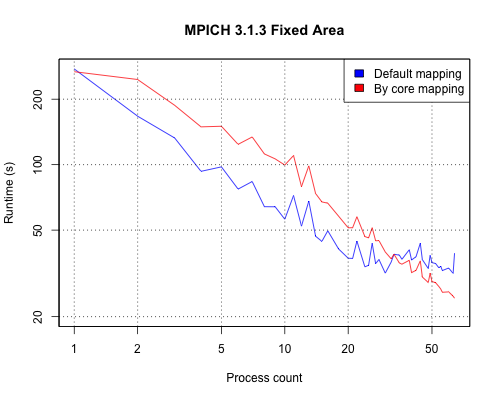
\includegraphics[width=0.5\textwidth]{images/MPICH313-fixed-area.png}
    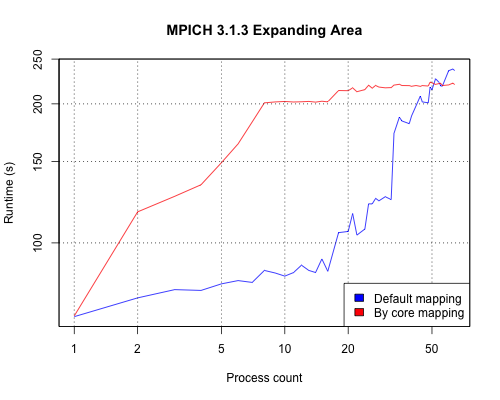
\includegraphics[width=0.5\textwidth]{images/MPICH313-expanding-area.png}
    \begin{itemize}
        \item MPI on togian
    \end{itemize}
}
\subsection{GMCF Shared-memory evaluation}
\frame{
    \frametitle{GMCF Shared-memory evaluation}
    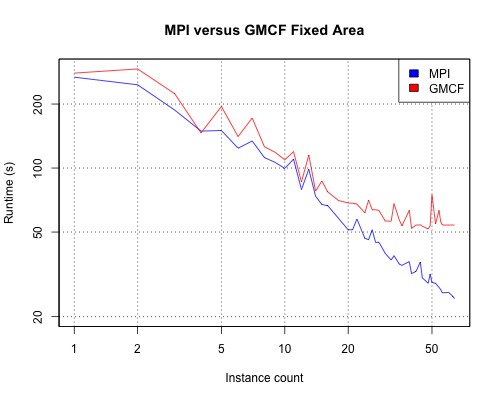
\includegraphics[width=0.5\textwidth]{images/GMCF-MPI-fixed-area.png}
    \includegraphics[width=0.5\textwidth]{images/GMCF-MPI-expanding-area.png}
    \begin{itemize}
        \item GMCF on togian
    \end{itemize}
}
\placelogotrue
\subsection{MPI Distributed-memory evaluation}
\frame{
    \frametitle{MPI Distributed--memory evaluation}
    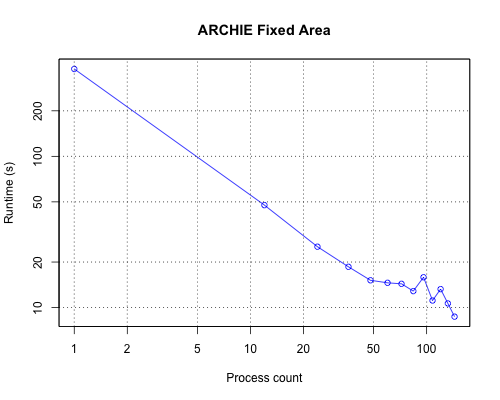
\includegraphics[width=0.5\textwidth]{images/ARCHIE-fixed-area.png}
    \includegraphics[width=0.5\textwidth]{images/ARCHIE-expanding-area.png}
    \begin{itemize}
        \item MPI on ARCHIE
    \end{itemize}
}
\placelogofalse
\section{GMCF Performance Improvements}
\frame{
    \frametitle{GMCF Performance Improvements}
    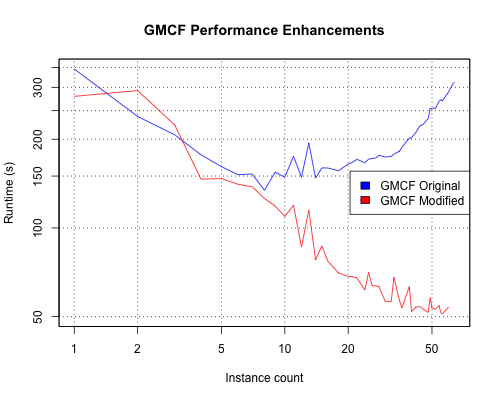
\includegraphics[width=0.5\textwidth]{images/GMCF-before-after-fixed-area.png}
    \begin{itemize}
        \item Was really bad, now better
        \item Global reduction
        \item Spin locks
        \item Thread pinning
        \item Other stuff
    \end{itemize}
}
\section{Conclusion}
\frame{
    \frametitle{Conclusion}
    \begin{itemize}
        \item GMCF competitive with MPI
        \item Future work to make it better
    \end{itemize}
}
\end{document}
